\chapter{Protótipo AFD e Plano de Testes}

Esse capítulo apresenta a arquitetura e a implementação de um protótipo para o AFD (Assentamento Funcional Digital) que objetiva servir para a investigação proposta nesse trabalho e descrita na introdução. Como o protótipo arquitetural foi baseado em uma arquitetura orientada a serviços ~\cite{erl:2007} que disponibiliza algumas das principais capacidades para manter os dados do AFD, iniciaremos o capítulo com a descrição de \textit{Web service}. Logo em seguida será descrita as principais características do projeto como tecnologias utilizadas e arquitetura proposta. Para finalizarmos o capítulo descrevemos os planos de testes que foram desenvolvidos para os testes de performance.

\section{Web-Service}


Nessa seção daremos uma visão de o que é \textit{web service}, e mostraremos um pouco sobre os seus principais componentes. Essa seção foi baseado no w3c schools ~\cite{w3cs} exeto quando citado explicitamente.

\subsection{O que é web-service?}

\textit{Web service} são componentes que podem ser acessados via protocolo http. Atualmente é muito usado na comunicação entre aplicações diferentes. O acesso a um \textit{web service} é via http, mas internamente existe dados formatados em xml que estão empacotados no protocolo SOAP (Simple Object Access Protocol).

Hoje várias aplicações podem acessar a web usando os \textit{browsers} e nem sempre essas aplicações conversam entre si. Para que a comunicação entre essas diversas aplicações se tornasse possível, independente da plataforma em que estivessem desenvolvidas, foi criado o conceito de \textit{web service}. Usando \textit{web services}, as aplicações podem publicar suas funções para toda a web. Usando o XML para codificar e SOAP para transportar os dados, os \textit{web services} elevaram as aplicações web para outro nível.

\subsection{Componentes de um Web-Service}

Um \textit{web service} é formado por três elementos: SOAP, WSDL e UDDI.

\subsubsection{SOAP}


O SOAP (Simple Object Access Protoco) é um protocolo leve para troca de informações que foi criado pela Microsoft, Ariba e IBM para padronizar a transferência de dados em diversas aplicações, por isso, se dá em XML. Parte da sua especificação é composta por um conjunto de regras de como utilizar o XML para representar os dados. Outra parte define o formato de mensagens, convenções para representar as chamadas de procedimento remoto (RPCs) utilizando o SOAP, e associações ao protocolo HTTP. 

SOAP é:

\begin{itemize}
	\item Um protocolo de comunição;
	\item É usado para a comunicação entre aplicações;
	\item É um padrão para envio de mensagens;
	\item Sua comunicação se dá na internet;
	\item É independente de plataforma;
	\item É independente de linguagem de programação;
	\item É baseado em XML;
	\item Permite passar por \textit{firewalls};
	\item É uma recomendação do W3C;
\end{itemize}

Atualmente as aplicações se comunicam via RPC (Remote Procedure Calls), mas o HTTP não foi desenhado para isso. RPC possui problemas de compatibilidade e segurança; \textit{firewalls} e servidores de \textit{proxy} normalmente bloqueiam mensagens desse tipo. Para resolver esses problemas foi criado o protocolo SOAP.

Uma mensagem SOAP (Exemplo \ref{listing:msgsoap}) é basicamente um documento XML que contem os seguintes elementos:

\begin{itemize}
	\item Um elemento 'Envelope' que identifica o documento XML como uma mensagem SOAP;
	\item Um elemento 'header' que contem informações de cabeçalho;
	\item Um elemento 'body' que contem informações de chamadas e retornos;
	\item Um elemento 'Fault' que contem informações sobre erros e status;
\end{itemize}


\definecolor{gray}{rgb}{0.4,0.4,0.4}
\definecolor{darkblue}{rgb}{0.0,0.0,0.6}
\definecolor{cyan}{rgb}{0.0,0.6,0.6}

\lstset{
  basicstyle=\ttfamily,
  columns=fullflexible,
  showstringspaces=false,
  commentstyle=\color{gray}\upshape
}

\lstdefinelanguage{XML}
{
  morestring=[b]",
  morestring=[s]{>}{<},
  morecomment=[s]{<?}{?>},
  stringstyle=\color{black},
  identifierstyle=\color{darkblue},
  keywordstyle=\color{cyan},
  morekeywords={xmlns,version,type}% list your attributes here
}


\lstset{language=XML}
\begin{lstlisting}[caption={Estrutura de uma mensagem SOAP},frame=trBL,breaklines=true,label=listing:msgsoap]
<?xml version="1.0"?>

<soap:Envelope
xmlns:soap="http://www.w3.org/2001/12/soap-envelope"
soap:encodingStyle="http://www.w3.org/2001/12/soap-encoding">

<soap:Header>
...
</soap:Header>

<soap:Body>
...  
	<soap:Fault>
	  ...  
	</soap:Fault>
</soap:Body>

</soap:Envelope>
\end{lstlisting}

\subsection{WSDL}

WSDL é uma linguagem baseada em XML para localizar e descrever \textit{web services}.

O WSDL (\textit{Web Services Description Language}) é uma linguagem baseada em XML, com a finalidade de documentar as mensagens que o Web service aceita e gera (Exemplo \ref{listing:wsdl}). É uma espécie de contrato. Esse mecanismo padrão facilita a interpretação dos 'contratos' pelos desenvolvedores e ferramentas de desenvolvimento. 

WSDL é:

\begin {itemize}
	\item A linguagem padrão para descrever \textit{web services};
	\item É baseado em XML;
	\item É usado para localizar \textit{web services};
	\item É um padrão W3C.
\end {itemize}

Um WSDL descreve um \textit{web service} usando pricipalmente os seguintes elementos:

\begin{table}[h]
	\caption{Elementos de um documento WSDL}
	\begin{center}
	\begin{tabular}{ccc}
		\hline
			\textbf{Elemento} & \textbf{Descrição} \\
		\hline
			<types> & Um container para a definição dos tipos de dados usados pelo \textit{web service}\\
			<message> & Definição dos dados que serão usados na comunicação \\
			<portType> & Um conjunto de operações suportadas por um ou mais \textit{endpoints} \\
			<binding> & Um protocolo e especificação de dados para um \textit{port type} específico\\
		\hline
	\end {tabular}
	\end{center}
	%\{Fonte: http://www.w3schools.com/}
	\label{tab:elementosWsdl}
\end{table}

Abaixo temos uma fração simplificada de um documento WSDL:

\lstset{language=XML}
\begin{lstlisting}[caption={WSDL},frame=trBL,breaklines=true,label=listing:wsdl]
<message name="getTermRequest">
  <part name="term" type="xs:string"/>
</message>

<message name="getTermResponse">
  <part name="value" type="xs:string"/>
</message>

<portType name="glossaryTerms">
  <operation name="getTerm">
    <input message="getTermRequest"/>
    <output message="getTermResponse"/>
  </operation>
</portType> 
\end{lstlisting}

\subsection{UDDI}

UDDI é um serviço de diretório que permite às empresas descobrir, registrar e procurar \textit{web services}. É baseado em padrões do W3C (\textit{World Wide Web Consortium}) e IETF (\textit{Internet Task Force}) como XML, HTTP e DNS.

Os benefícios de se usar UDDI são muitos. Antes do UDDI não havia padrão para as empresas divulgarem seus produtos e serviços para os seus consumidores e parceiros. Com o UDDI, por exemplo, se for definido um padrão para serviços de empresas aéreas, quando as empresas publicarem os seus serviços em um diretório UDDI as agências de viagem poderão procurar por esses serviços e iniciar imediatamente a comunicação.














\section{O Protótipo}

Para a execução dos testes de performance foi desenvolvido uma aplicação orientada a serviços ~\cite{erl:2007} com as principais capacidades necessárias para manter os dados do AFD. O objetivo central da aplicação é manter os documentos da pasta funcional dos servidores. Como a aplicação deve armazenar aquivos, escolhemos gravar o arquivo no sistema operacional e armazenar o caminho para ele na base de dados. O objetivo ao se escolher realizar os testes de performance em uma arquitetura orientada a serviços foi o de flexibilizar ao máximo as implementações em diversos bancos de dados. Na tabela \ref{tab:funcionalidades} a descrição das funcionalidades implementadas.

\renewcommand{\arraystretch}{3}

\begin{table}
	\caption{Descrição das Funcionalidades}
	\begin{center}
	\begin{tabularx}{\textwidth}{ | c | X | }
		\hline
			\textbf{Funcionalidade} & \multicolumn{1}{c|}{\textbf{Descrição}} \\
		\hline
			Insere Orgão & \noindent\parbox[c]{\hsize}{Permite inserir as unidades pagadoras ou orgãos que terão os dados dos empregados mantidos no sistema.} \\
		\hline
			Insere Empregado & \noindent\parbox[c]{\hsize}{Permite inserir os empregados de cada orgão.} \\
		\hline
			Insere Dependente & \noindent\parbox[c]{\hsize}{Permite inserir os dependentes de cada empregado.}\\
		\hline
			Insere Documento Dependente & \noindent\parbox[c]{\hsize}{Permite inserir os documentos dos dependentes que farão parte da pasta funcional do empregado.} \\
		\hline
			Insere Documento Empregado & \noindent\parbox[c]{\hsize}{Permite inserir os documentos que farão parte da pasta funcional do empregado.} \\
		\hline
			Lista Orgãos & \noindent\parbox[c]{\hsize}{Lista os dados dos órgãos cadastrados no sistema.} \\
		\hline
			Lista Empregados & \noindent\parbox[c]{\hsize}{Lista os dados dos empregados cadastrados no sistema.} \\
		\hline
			Lista Dependentes & \noindent\parbox[c]{\hsize}{Lista os dados dos dependentes dos empregados.} \\
		\hline
			Lista Documentos Empregados & \noindent\parbox[c]{\hsize}{Retorna os documentos da pasta funcional do empregado.} \\
		\hline
			Lista Documentos Dependentes & \noindent\parbox[c]{\hsize}{Retorna os documentos dos dependentes dos empregados.} \\
		\hline
			Relatório de Empregados Ativos & \noindent\parbox[c]{\hsize}{Calcula e exibe a quantidade de empregados ativos por orgão.} \\
		\hline
			Lista Vínculos & \noindent\parbox[c]{\hsize}{Lista os valores possíveis para os tipos de vínculos entre empregados e dependentes.} \\
		\hline
			Lista Tipo Documentos & \noindent\parbox[c]{\hsize}{Lista os valores possíveis para os tipos de documentos.} \\
		\hline
			Remove Dependente & \noindent\parbox[c]{\hsize}{Exclui o depente e seus arquivos.} \\
		\hline
			Desliga Empregado & \noindent\parbox[c]{\hsize}{Atualiza o status do empregado incluindo a data de desligamento.} \\
		\hline
	\end {tabularx}
	\end{center}
	%\caption{Fonte: http://docs.mongodb.org}
	\label{tab:funcionalidades}
\end{table}

\section{A Arquitetura do Projeto}

Para cumprirmos o nosso objetivo, que é testar a aplicação com diferentes bancos de dados, montamos uma arquitetura simples, mas que nos permite trocar as implementações da camada de persistência sem maiores esforços. Para a execução dos testes utilizamos o JMeter. A aplicação foi desenvolvida em Python com o apoio do framework web2py na implementação do \textit{web service}. A linguagem de programação Python foi escolhida pela facilidade de encontrar drivers de diversos bancos de dados relacionais e não relacionais, além de ser uma linguagem orientada a objetos e de ampla utilização. O framework web2py foi adicionado ao projeto pelo motivo de suportar a implementação de \textit{web services} de modo rápido e fácil, além da geração automática do WSDL (arquivo que contém a descrição das operações do Web service). A diagramação da arquitetura pode ser vista na figura \ref{fig:arquitetura}

	\begin{figure}[!htbp]
		\begin{center}
			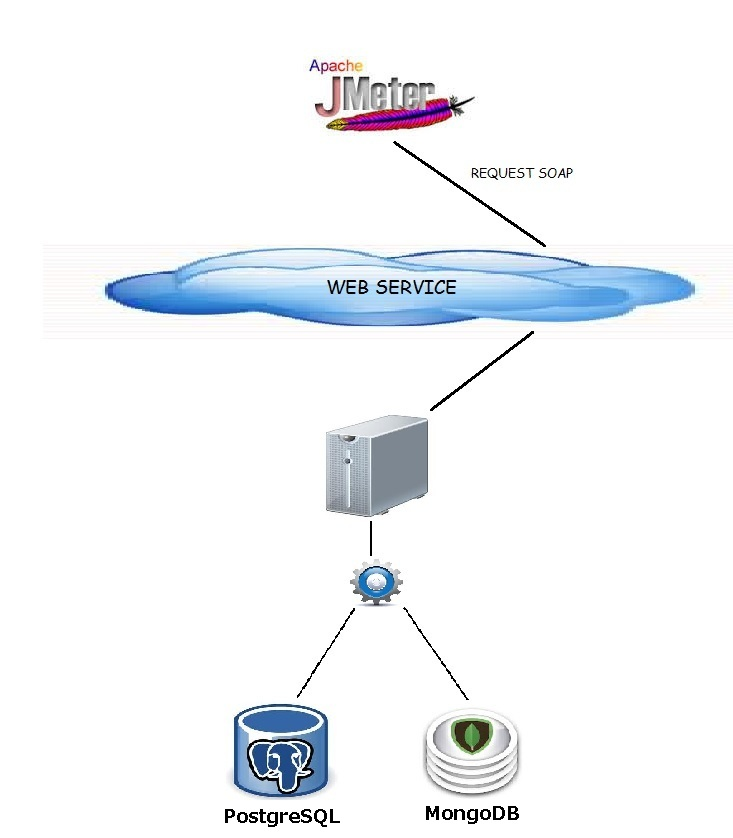
\includegraphics[width=0.5\textwidth]{arquitetura}
		\end{center}
		\caption{Arquitetura de Testes}
		\label{fig:arquitetura}
	\end{figure}

\subsection{web2py}

Web2py é um \textit{framework} para desenvolvimento ágil de aplicações web, software livre e gratuito. Ele é escrito e programável em Python. web2py foi inspirado pelo Ruby on Rails e Django. Tem seu foco no desenvolvimento ágil e segue o MVC (\textit{Model View Controller}). Toda aplicação web2py é composta por \textit{Models} (arquivos que contem a descrição dos dados), \textit{Views} (arquivos que contem a descrição dos dados que serão apresentados), \textit{Controlers} (arquivos que contem a lógica e \textit{workflow} do negócio), \textit{Cron Jobs} (tarefas que precisam ser executadas regularmente) e \textit{Static Files} (imagens, \textit{scripts}, folhas de estilos, etc.) ~\cite{siteweb2py}.

Quando se trata de Web services, web2py oferece suporte para diversos protocolos, incluindo XML, JSON, RSS,CSV,XMLRPC,JSONRPC,AMFRPC, e SOAP.  O web2py inclui um cliente e servidor SOAP (pysimplesoap) criado por Mariano Reingart. Uma facilidade encontrada é a geração automática do WSDL e da página com a descrição das capacidades ~\cite{siteweb2py}.

\section{Os Planos de Teste}

Foi desenvolvido um plano de testes no JMeter para a maioria das funcionalidade da nossa aplicação. Os testes serão individualmente discutidos na seção de resultados do próximo capítulo. O testador utilizado no nosso projeto foi o de Requisição SOAP/XML - RPC. É nele que configuramos as requisições que serão feitas ao Web service da aplicação. Além de configurar uma requisição para cada plano de teste, temos como parametrizar outras configurações como a quantidade de usuários virtuais e o intervalo entre a inicialização de cada usuário. Na tabela \ref{tab:configplanoteste} temos as principais configurações dos nossos planos de teste. É importante realçar que todas as capacidades da nossa aplicação foram desenvolvidas para validarem os dados da mesma forma, ou seja, as regras de negócio verificadas, tanto usando o mongodb quanto o postgresql, são as mesmas. O passo a passo da execução dos planos de testes se dividem em dois tipos: Inserção/Exclusão/Atualização e Consulta.

\begin{table}
	\caption{Principais configurações dos Planos de Teste}
	\begin{center}
	\begin{tabularx}{\textwidth}{ | c | X | }
	\hline
		\textbf{Parâmetro} & \multicolumn{1}{c|}{\textbf{Descrição}} \\
	\hline
		Quantidade de usuários virtuais (threads) & Quanto maior o número de usuários virtuais, maior será o número de requisições simultâneas que a nossa aplicação terá que responder.\\
	\hline 
		Tempo de inicialização dos usuários virtuais & Indica o tempo total para a inicialização de todos os usuários virtuais. Para encontrarmos o tempo entre a inicialização de cada usuário devemos dividir pelo total de usuários virtuais.\\
	\hline
		O local dos arquivos CSV & Esses arquivos devem ser gerados antes do início dos testes com o apóio de um script.\\
	\hline
		Intervalo de medição dos gráficos & É o intervalo de tempo em que o JMeter faz as medidas para plotar cada gráfico.\\
	\hline
	\end {tabularx}
	\end{center}
	\label{tab:configplanoteste}
\end{table}

\subsection{Planos de Teste de Inserção/Exclusão/Atualização}

Os planos de Testes de Inserção executam os seguintes passos:

\begin{enumerate}
\item Configuração de Dados CSV - É indicado onde está o arquivo csv de onde as threads lerão os valores a serem enviados na requisição soap;
\item Requisição SOAP/XML-RPC - É configurada a URL do Web service e a requisição que será realizada. Cada requisição será montada com os dados lidos do arquivo csv. Cada thread lê uma linha diferente do arquivo.
\item Gráfico de Tempo de Resposta -  Elemento responsável por gerar um gráfico a partir dos dados da requisição feita. O gráfico exibe a  evolução do tempo de resposta das requisições feitas.
\item Gráfico de Resultados - Elemento responsável por exibir a evolução dos tempos das requisições, a média dos tempos das requisições, a derivação do tempo das requisições e a vazão.
\end{enumerate}

As funcionalidades que seguem esses passos são: insere órgão, insere empregado, insere dependente, insere documento dependente, insere documento empregado, desliga empregado e remove dependente.

Os testes que manipulam os arquivos da pasta funcional, devido à limitação da arquitetura disponível, e o teste de inserção de órgãos, devido a baixa massa de dados, só foram realizados para 10 e 100 usuários simultâneos. O restante foi executado para 10, 100 e 500 usuários simultâneos

\subsection{Planos de Teste de Consulta}

Os planos de Testes de Consulta executam os seguintes passos:

\begin{enumerate}
\item Requisição SOAP/XML-RPC - É configurada a URL do Web service e a requisição que será realizada. Cada requisição será montada com os dados lidos do arquivo csv. Cada thread lê uma linha diferente do arquivo.
\item Gráfico de Tempo de Resposta -  Elemento responsável por gerar um gráfico a partir dos dados da requisição feita. O gráfico exibe a  evolução do tempo de resposta das requisições feitas.
\item Gráfico de Resultados - Elemento responsável por exibir a evolução dos tempos das requisições, a média dos tempos das requisições, a derivação do tempo das requisições e a vazão.
\end{enumerate}

As funcionalidades que seguem esses passos são: lista órgãos, lista empregados, lista dependentes, lista documentos dos empregados, lista documentos dos dependentes e relatório de empregados ativos.

Cada plano de teste de consulta foi executado durante um minuto. Os testes que manipulam os arquivos da pasta funcional, devido à limitação da arquitetura disponível, só foram realizados para 10 e 100 usuários simultâneos. O restante foi executado para 10,100 e 500 usuários simultâneos.